%% 第一章 绪论

\chapter{绪论}
\chaptermark{绪论}

\section{研究背景}

近年来，随着大语言模型（Large Language Models，LLMs）\cite{vaswani2017attention,brown2020gpt3}与多模态感知技术的快速发展，服务机器人正逐步由实验室验证阶段走向家庭服务、医疗辅助、物流配送以及人机协作等长期开放场景。与工业机器人主要在结构化环境中执行重复性任务不同，服务机器人需要在动态环境下持续运行，并通过自然语言与用户进行长期交互。因此，机器人不仅需要具备完成即时任务的能力，还需要能够对过去经历进行理解、回忆与表达，从而回答诸如"上周完成了什么任务""某个物体曾经放置于何处""某次任务失败的原因是什么"等回溯性问题。

这种将机器人历史经历组织并转化为自然语言问答的能力，被称为情景记忆语言化（Episodic Memory Verbalization，EMV）\cite{tulving1972episodic,liu2024hemv}。情景记忆语言化不仅关系到机器人对历史信息的管理能力，也直接影响人机交互过程中的可解释性、可信性与长期协作体验。随着机器人部署时间不断增长，系统需要处理的历史经历规模将迅速扩大，如何在海量历史数据中高效定位与当前问题相关的关键信息，已成为长期机器人系统中的重要研究问题。

面向长期情景记忆问答，当前系统主要面临以下三个方面的挑战。

（1）检索效率与历史规模增长之间的矛盾。随着机器人持续运行，其积累的经历数据会不断增长，历史长度可能由数小时扩展至数周甚至数月。在长时间运行条件下，系统需要从大量历史经历中快速定位与当前问题相关的少量关键证据。若直接将全部历史输入语言模型，不仅会带来较高的计算与存储开销，也容易导致模型在长序列条件下出现信息利用效率下降的问题。

（2）存储开销与信息保留之间的矛盾。服务机器人在运行过程中会持续产生大量多模态数据，包括图像、音频、动作序列以及场景关系等信息。若对所有历史数据进行长期完整保存，系统存储规模将随运行时间持续增长；而若采用简单的时间窗口删除策略，又可能导致关键历史细节的丢失，从而影响后续回溯性问答的准确性。

（3）记忆固定性与错误修正需求之间的矛盾。机器人在感知、场景理解以及语言摘要过程中不可避免地会产生识别误差或语义偏差。当这些错误被写入记忆结构后，可能进一步影响后续问答结果，甚至在层级摘要过程中逐渐传播与放大。因此，长期记忆系统不仅需要具备记忆能力，还需要具备一定的动态修正与维护能力。

针对长历史记忆问答问题，现有研究主要形成了三类技术路线。

第一类为长上下文语言模型方案\cite{brown2020gpt3,achiam2023gpt4,gemini2023gemini,reid2024gemini}。该类方法利用具有较大上下文窗口的大语言模型，将机器人完整历史记录直接输入模型，由模型在全局上下文中完成推理与答案生成。该方法实现方式较为直接，但随着历史长度增加，模型输入规模与推理成本会迅速增长。此外，已有研究表明，长上下文模型在长序列中部区域的信息利用能力相对有限，容易出现"中间信息丢失"现象\cite{liu2024lost}。

第二类为检索增强生成（Retrieval-Augmented Generation，RAG）方案\cite{lewis2020rag}。该类方法首先对历史记录进行切分与向量化表示，再根据语义相似度检索与当前问题相关的历史片段，仅将少量检索结果输入语言模型生成答案。该方案能够有效降低 token 消耗，但在涉及跨时间、跨任务的复杂回溯问题时，仅依赖文本语义相似度可能难以覆盖所有相关证据。

第三类为层级记忆方案\cite{liu2024hemv}。该类方法通过多层摘要结构对机器人经历进行组织，并借助大语言模型智能体（LLM Agent）对层级结构进行展开、折叠与搜索，从而实现长历史记忆检索。相较于前两类方案，层级记忆方法在控制上下文规模方面具有一定优势，但现有研究更多关注"如何检索历史"，对于长期运行中的记忆维护问题仍缺乏系统研究。例如，层级树结构主要表达纵向父子关系，难以直接支持跨节点的横向关联；记忆通常以追加式方式增长，长期运行后容易导致存储规模持续膨胀；同时，摘要一旦生成后往往难以修正，错误信息可能在层级结构中逐渐传播。

\begin{figure}[htbp]
    \centering
    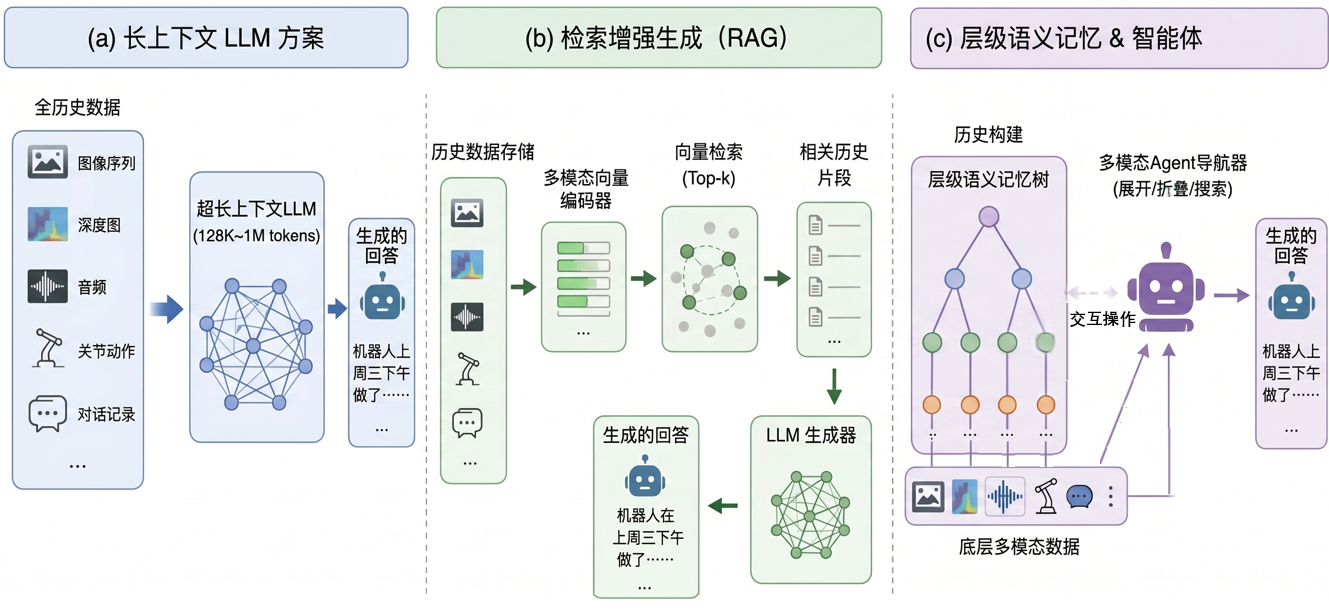
\includegraphics[width=\textwidth]{content/figures/图1-1 长历史具身情景记忆问答主要技术路线对比.png}
    \caption{长历史具身情景记忆问答主要技术路线对比}
    \label{fig:tech-routes}
\end{figure}

因此，面向长期部署的机器人情景记忆系统，不仅需要具备高效的历史检索能力，还需要具备主动的记忆维护能力，包括选择性遗忘、结构化组织以及错误修正等功能。如何在保证问答准确性的同时，提高长期运行条件下系统的可扩展性与可维护性，是当前长期机器人记忆研究中的重要问题。

\section{研究现状}

服务机器人是一类在非结构化环境中为人类提供辅助服务的自主系统，其应用场景涵盖家庭陪护、医疗康复、物流配送以及人机协作等多个领域\cite{siciliano2016robotics,broadbent2017service,thrun2005probabilistic,waibel2011roboearth}。与工业机器人在结构化环境中执行重复性任务不同，服务机器人需要在动态、开放的环境中持续运行，并通过自然语言与用户进行长期交互。在长期运行场景中，机器人不仅要完成即时操作任务，还需要持续积累和管理大量历史经历，以便在用户提出回溯性问题时从长期记忆中提取相关证据并生成可解释的答案。因此，长期情景记忆已成为服务机器人实现长期自主交互的核心基础能力之一。

近年来，基于自然语言表示的记忆方法逐渐受到广泛关注。与基于固定向量编码的端到端记忆方法相比，自然语言记忆表示具有更强的可解释性与可扩展性，同时大语言模型（LLM）的零样本与少样本推理能力使其能够直接基于自然语言记忆完成复杂问答任务。在长历史记忆问答方面，现有研究主要形成了三类技术路线。

\textbf{长上下文语言模型方案}利用具备超长上下文窗口的 LLM 直接将完整历史记录输入模型进行端到端推理\cite{achiam2023gpt4,reid2024gemini}。该类方法实现较为直接，但随着历史长度增长，推理成本迅速攀升，且已有研究表明长上下文模型在长序列中部区域存在信息利用效率下降的问题\cite{liu2024lost}。

\textbf{检索增强生成方案}首先对历史进行切分与向量化，根据语义相似度检索相关片段后输入模型生成答案\cite{lewis2020rag}。该方案能有效降低 token 消耗，但在涉及跨时间、跨任务的复杂回溯问题时，仅依赖文本语义相似度难以覆盖所有相关证据。

\textbf{层级记忆方案}通过多层摘要结构组织机器人经历，借助 LLM 智能体对层级树进行展开、折叠与搜索\cite{liu2024hemv}。H-EMV 框架将连续经历逐步压缩为不同层级的自然语言摘要，在控制上下文规模方面具有一定优势，但其在长期部署中仍面临三个主要局限：（1）层级树结构主要表达纵向父子关系，对跨时间、跨目标的横向语义关联支持不足；（2）记忆以追加方式持续增长，缺乏主动的存储管理机制，长期运行后存储规模不断膨胀；（3）摘要生成后缺乏有效的动态修正手段，感知或理解偏差一旦写入便可能在层级结构中传播与放大。

在记忆压缩与遗忘方面，现有工作主要借鉴认知科学中的遗忘曲线理论。艾宾浩斯遗忘曲线描述了人类记忆随时间指数衰减的规律，一些研究将其引入对话系统的长期记忆管理\cite{packer2023memgpt}。然而，现有遗忘策略大多仅依赖时间维度，缺乏对记忆内容价值的多维评估。在机器人场景中，一段包含用户关键指令的对话经历即使时间久远也远比近期的重复导航帧更有保留价值，仅靠时间衰减难以做出合理的压缩决策。

在记忆修正方面，现有方法主要集中在知识编辑领域，通过对模型参数或表示的局部修改来更新事实知识\cite{meng2022rome,mitchell2022fast}。这些方法面向模型内部知识的修正，而长期机器人记忆中的错误往往嵌入在结构化的经历数据中，且可能在层级摘要间传播，需要从数据层面进行定位与修复。

综上所述，当前长期机器人记忆研究在检索效率、存储管理与错误修正三个维度上仍缺乏系统性的整合方案。本文在层级记忆树的基础上，分别从图增强检索、效用引导遗忘和反馈驱动修正三个方面展开研究，构建一个面向长期部署的主动式情景记忆维护框架。

\section{研究目的与研究内容}

针对长期机器人经验问答中存在的检索效率不足、记忆持续膨胀以及错误传播等问题，本文提出一种面向长期部署场景的主动式层级情景记忆框架 \textbf{GRAF-Mem}（Graph-Retrieval and Adaptive Forgetting Memory）。该框架在保留层级记忆树纵向组织结构的基础上，引入图增强检索、效用引导遗忘以及反馈驱动修正机制，以提升长期记忆系统的整体可维护性与长期运行能力。

本文的主要研究内容如下。

\textbf{（1）图增强检索与结构化问答方法研究。}针对层级树结构横向语义关联能力不足的问题，本文研究基于事件关联图的图增强检索方法。通过构建事件之间在时间、对象、位置以及动作等维度上的关联关系，增强跨节点证据发现能力，提高复杂回溯性问题中的检索召回率与问答准确性。

\textbf{（2）效用引导的渐进式遗忘方法研究。}针对长期运行过程中记忆规模持续增长的问题，本文研究基于记忆效用评估的渐进式遗忘机制。该机制综合考虑记忆的新近性、重要性与独特性，对不同类型的历史信息采用差异化保留与压缩策略，从而在控制存储规模的同时尽可能保留关键历史信息。

\textbf{（3）反馈驱动的记忆修正方法研究。}针对长期记忆中错误信息难以修正的问题，本文研究基于反馈信息的记忆修正机制。通过对可能存在错误的记忆节点进行定位与修正，并结合关联关系分析错误传播范围，从而降低错误信息对后续问答结果的影响。

总体而言，本文希望从检索、存储与维护三个层面对长期情景记忆系统进行改进，使机器人记忆系统不仅能够支持长历史问答，还能够适应长期部署场景下持续变化的环境与交互需求。

\begin{figure}[htbp]
    \centering
    
\includegraphics[width=\textwidth]{图1-2 GRAF-Mem总体框架图.png}
    \caption{GRAF-Mem 总体框架图}
    \label{fig:graf-arch}
\end{figure}

\section{本文内容安排}

本文共分为六章，各章节内容安排如下。

\textbf{第一章为绪论。}介绍服务机器人长期部署背景下情景记忆研究的意义，分析长期情景记忆面临的主要问题，综述国内外研究现状，并给出本文的研究目标与主要研究内容。

\textbf{第二章为相关工作。}主要从机器人情景记忆、长历史问答、图增强检索、记忆压缩与遗忘以及记忆修正等方面，对国内外相关研究进行综述与分析。

\textbf{第三章为图增强检索与结构化问答。}介绍事件关联图的构建方法、图增强检索流程以及结构化检索机制，并验证其在长历史问答任务中的有效性。

\textbf{第四章为效用引导的渐进式遗忘。}介绍记忆效用评估方法、分级遗忘策略以及安全机制，并分析该方法在存储压缩与问答性能保持方面的效果。

\textbf{第五章为反馈驱动记忆修正。}介绍错误定位、摘要修正以及传播检测等方法，并验证该机制在降低错误传播方面的有效性。

\textbf{第六章为总结与展望。}总结全文研究工作与主要实验结果，并对未来研究方向进行展望。
